% =============================================================================
% ICCCIoT-2026 / IC3IoT-2026 submission
% Track 4: Blockchain, Cloud Computing and Big Data Analytics
%
% SUBMISSION FACTS (verified 2026-08-02; re-check the live site before upload):
%   - Extended submission deadline: 04 August 2026
%   - Notification: 01 Sep 2026 | Camera-ready: 10 Sep 2026 | Conf: 24-25 Sep 2026
%   - Page limit: 6 pages incl. references; extra pages are charged
%   - Similarity ceiling: <= 20% (Turnitin/iThenticate)
%   - Review is DOUBLE-BLIND -- keep \blindreviewtrue for the review copy
%   - Portal: https://cmt3.research.microsoft.com/ICCCIOT2026
%     (the conference site's own footer links a STALE 2024 portal -- ignore it)
%
% All numeric results are \input from paper/tables/*.tex, generated by
% src/tables.py from results/. No number in this file is typed by hand.
% =============================================================================

\documentclass[conference,10pt,letterpaper]{IEEEtran}

\usepackage{cite}
\usepackage{amsmath}
\usepackage{amssymb}
\usepackage{amsfonts}
\usepackage{algorithm}
\usepackage{algpseudocode}
\usepackage{graphicx}
\usepackage{textcomp}
\usepackage{xcolor}
\usepackage{array}
\usepackage{booktabs}
\usepackage{url}

\newif\ifblindreview
\blindreviewtrue   % <-- SET TO \blindreviewfalse ONLY for camera-ready

% Break chosen so both lines fit the measure; a longer first line silently
% wraps and strands a single word on its own line.
\title{Prefill Dominates: Content-Blind Work-Aware\\
Scheduling for LLM Inference Serving}

\ifblindreview
  \author{\IEEEauthorblockN{Anonymous Author(s)}
  \IEEEauthorblockA{Affiliation withheld for double-blind review}}
\else
  \author{
    \IEEEauthorblockN{1\textsuperscript{st} Given Name Surname}
    \IEEEauthorblockA{\textit{Department} \\ \textit{Institution}\\ City, Country \\ email@example.edu}
    \and
    \IEEEauthorblockN{2\textsuperscript{nd} Given Name Surname}
    \IEEEauthorblockA{\textit{Department} \\ \textit{Institution}\\ City, Country \\ email@example.edu}
  }
\fi

\begin{document}
\maketitle

\begin{abstract}
Large language model (LLM) inference services schedule requests without knowing
how many tokens each will generate. Because a long response occupies a batch
slot for many iterations, first-come-first-serve scheduling suffers severe
head-of-line blocking, and a substantial literature therefore predicts output
length from the \emph{prompt text} in order to approximate shortest-job-first.
Reading prompt content, however, is precisely what a privacy-constrained or
regulated serving platform cannot do. We ask how much of that benefit survives
if the scheduler is forbidden to inspect prompts. Analysing 44.1 million
requests from Microsoft Azure's production LLM inference traces, we find that
the premise of the length-prediction literature does not hold for these
workloads: prefill, which is \emph{exactly observable} at admission from the
context length alone, accounts for 91.2\% and 98.7\% of total schedulable work
in the conversation and code workloads respectively, while the unobservable
decode component accounts for the remainder. We propose CB-SJF-Work, a
content-blind scheduler that orders admissions by estimated total service work
using only token counts and arrival metadata. Across five disjoint windows of
production traffic, CB-SJF-Work reduces mean normalised latency by up to 73.0\%
over first-come-first-serve and recovers 92.5\% (conversation) and 78.5\% (code)
of the improvement attainable by an oracle with perfect knowledge of output
length. Notably, it does so on the code workload even though output length there
is essentially unpredictable from metadata (Spearman $\rho_s=0.073$), and it
outperforms a scheduler driven by an explicit learned length predictor. The
widely assumed privacy--performance tradeoff in LLM request scheduling is, for
these production workloads, largely illusory.
\end{abstract}

\begin{IEEEkeywords}
LLM inference serving, cloud scheduling, head-of-line blocking, privacy-preserving
systems, production trace analysis, big data architectures
\end{IEEEkeywords}

% ============================================================================
\section{Introduction}
\label{sec:intro}

Serving large language models has become one of the dominant consumers of cloud
GPU capacity. A modern inference engine such as vLLM~\cite{kwon2023pagedattention}
or Orca~\cite{yu2022orca} executes requests with \emph{continuous batching}: many
requests share a batch, and each scheduling iteration emits one token for every
request currently resident. A request occupies its slot, and its share of the
key--value (KV) cache, until it has produced its final token.

This creates a scheduling problem with an unusual information structure. The
duration for which a request will hold its slot is proportional to its output
length, and that length is \emph{not known when the request arrives}. Under
first-come-first-serve (FCFS), the default in production engines, a single
long-generating request admitted early can block many short ones behind it,
producing head-of-line (HOL) blocking and long tail latencies.

The established response is to predict the output length and then approximate
shortest-job-first (SJF). $S^3$ fine-tunes a DistilBERT model on the prompt to
predict sequence length~\cite{jin2023s3}; more recently, Fu \emph{et al.} learn
to rank requests by predicted output length, again from prompt
text~\cite{fu2024ltr}. Both report large gains. Both require the scheduler to
read the user's prompt.

That requirement is a genuine obstacle. A serving platform operating under
data-protection obligations, serving regulated sectors, or offering
confidential-computing guarantees may be contractually or legally unable to
route prompt content into a scheduling component, and running an auxiliary
transformer over every prompt also consumes the very accelerator capacity the
scheduler is trying to conserve. This motivates our question:

\begin{quote}
\emph{How much of the achievable scheduling benefit remains available to a
scheduler that never reads prompt content?}
\end{quote}

We answer it empirically on Microsoft Azure's public production LLM inference
traces~\cite{azurepublicdataset}, comprising 44.1 million real requests across a
conversation workload and a code workload. Our central finding is that the
question's premise --- that the valuable information is locked inside the prompt
--- is largely false for these workloads. Service time in a continuous-batching
engine has two components: a prefill pass over the input tokens, and a sequence
of decode iterations. The prefill cost is determined by the context length,
which \emph{is} visible at admission without reading a single token of content.
On the Azure traces, prefill accounts for 91.2\% and 98.7\% of total schedulable
work. The unobservable part is the small part.

We make the following contributions.

\begin{enumerate}
\item A characterisation of 44.1M production LLM inference requests showing that
      schedulable work is overwhelmingly prefill-dominated, and that output
      length is predictable from content-blind metadata for conversational
      traffic ($\rho_s = 0.384$) but effectively unpredictable for code
      completion ($\rho_s = 0.073$) --- despite the latter having the heavier
      output-length tail (Section~\ref{sec:characterisation}).
\item CB-SJF-Work, a content-blind admission policy that orders requests by
      estimated \emph{total service work} rather than by predicted output
      length, using only token counts and arrival metadata
      (Section~\ref{sec:method}).
\item A trace-driven evaluation against FCFS, two content-blind baselines and
      two oracles, over five disjoint windows of production traffic and five
      offered-load levels (Sections~\ref{sec:setup}--\ref{sec:results}).
      CB-SJF-Work recovers 92.5\% and 78.5\% of the attainable oracle
      improvement, and \emph{outperforms} an explicit learned length predictor.
\item The negative result that scheduling by predicted output length --- the
      objective adopted by prior work --- is actively harmful on the code
      workload, where it is worse than FCFS.
\end{enumerate}

% ============================================================================
\section{Background and Related Work}
\label{sec:related}

\textbf{Continuous-batching inference engines.}
Orca~\cite{yu2022orca} introduced iteration-level scheduling, and
vLLM~\cite{kwon2023pagedattention} added paged KV-cache management, together
establishing the execution model we assume: a batch whose membership changes
every iteration, bounded by GPU memory available for the KV cache.
Sarathi-Serve~\cite{agrawal2024sarathi} reduces prefill-induced decode stalls by
chunking prefills, and Splitwise~\cite{patel2024splitwise} and
DistServe~\cite{zhong2024distserve} disaggregate the two phases onto separate
hardware. These works change \emph{where and how} prefill and decode execute;
they are orthogonal to, and composable with, the question of \emph{which
request to admit next}, which is our subject.

\textbf{Output-length prediction for scheduling.}
$S^3$~\cite{jin2023s3} predicts output length with a fine-tuned DistilBERT to
reserve KV memory more tightly. Fu \emph{et al.}~\cite{fu2024ltr} observe that
exact lengths are unnecessary and learn only the relative \emph{rank} of output
lengths, reporting substantial latency reductions. Both extract their signal
from prompt text. Our work shares their diagnosis of HOL blocking but inverts
their prescription: we show that for production traces the dominant schedulable
quantity is already visible without the prompt.

\textbf{Production trace analysis.}
Characterising real cloud workloads has repeatedly overturned assumptions formed
on synthetic ones, as with Resource Central for VM
allocation~\cite{cortez2017resource} and Serverless in the Wild for
FaaS~\cite{shahrad2020serverless}. The Azure LLM inference
traces~\cite{azurepublicdataset} were released alongside
Splitwise~\cite{patel2024splitwise} and DynamoLLM~\cite{stojkovic2025dynamollm},
the latter using them for energy-aware cluster reconfiguration. We use them to
study admission ordering, and to our knowledge this is the first analysis of the
\emph{observability} of schedulable work in these traces.

% ============================================================================
\section{Characterising Production LLM Traffic}
\label{sec:characterisation}

\subsection{Traces}
We use the Azure LLM Inference Trace 2024~\cite{azurepublicdataset}, released
under CC-BY-4.0/MIT. It contains two one-week traces from Microsoft's production
inference service: a \emph{conversation} workload (27.3M requests) and a
\emph{code} workload (16.8M requests). Each record gives an arrival timestamp,
the input context length in tokens, and the number of tokens generated. Crucially
for our purpose, the traces contain \emph{no prompt text} --- they are themselves
a content-blind view of the workload, which is exactly the information a
privacy-constrained scheduler would possess.

\subsection{Schedulable work is prefill-dominated}
In a continuous-batching engine, servicing a request costs a prefill pass
proportional to its context length $x_i$, plus $y_i$ decode iterations where
$y_i$ is its output length. Charging decode at its marginal per-token cost
(the per-iteration base cost is a property of the batch, not of any one
request), the total work attributable to request $i$ is

\begin{equation}
  \label{eq:work}
  W_i \;=\; c_f \;+\; c_p\,x_i \;+\; c_d\,y_i ,
\end{equation}

\noindent where $c_p$ is the per-token prefill cost, $c_d$ the marginal
per-token decode cost, and $c_f$ a fixed overhead. The first two terms are known
at admission; only the third requires knowing $y_i$.

Fig.~\ref{fig:work} shows how that total divides on the real traces. Prefill
accounts for 91.2\% of schedulable work in the conversation trace and 98.7\% in
the code trace. The reason is visible in Table~\ref{tab:workloads}: mean context
lengths are 1632 and 2511 tokens, while mean output lengths are only 106 and 23.
Production traffic is dominated by long prompts and short completions --- a
regime in which the unobservable component of service time is small.

\begin{figure}[!t]
  \centering
  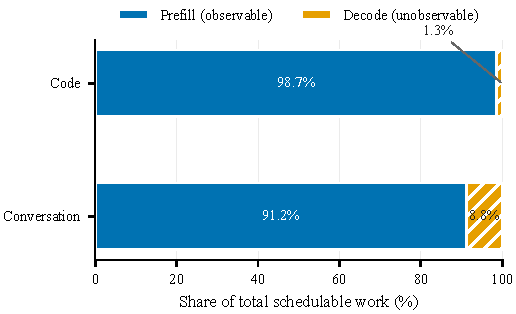
\includegraphics[width=\columnwidth]{../figures/fig1_work_breakdown.pdf}
  \caption{Composition of schedulable work in the Azure production traces.
  The prefill component is exactly observable at admission from the context
  length; the decode component requires knowing the output length, which is not
  available until the request completes.}
  \label{fig:work}
\end{figure}

% Auto-generated by src/tables.py -- do not edit by hand.
\begin{table}[!t]
\caption{Azure production trace characteristics. Prefill share is the fraction
of total schedulable work that is exactly observable at admission time.
$\rho_s$ and pairwise accuracy measure how well the content-blind predictor
recovers true output length.}
\label{tab:workloads}
\centering
\begin{tabular}{@{}lrrrrrr@{}}
\toprule
 & & \multicolumn{2}{c}{Mean tokens} & Prefill & \multicolumn{2}{c}{Predictor} \\
\cmidrule(lr){3-4}\cmidrule(lr){6-7}
Workload & Reqs. & Ctx. & Out. & share (\%) & $\rho_s$ & Pair.\ acc. \\
\midrule
Conversation & 27.3M & 1632 & 106 & 91.2 & 0.365 & 0.633 \\
Code & 16.8M & 2511 & 23 & 98.7 & 0.107 & 0.537 \\
\bottomrule
\end{tabular}
\end{table}


\subsection{Output length is not equally predictable}
Fig.~\ref{fig:pred} plots mean output length against context-length decile. For
conversational traffic the relationship is strong and monotone above the fourth
decile: mean output rises roughly ninefold across deciles, so context length
carries real information about output length. For code completion the curve is
flat --- output length is statistically independent of input length.

This matters because the two workloads have opposite risk profiles. The code
trace has both the heavier output-length tail and the weaker predictive signal:
it is the workload that would benefit most from length-aware scheduling and the
one where predicting length is hardest. A method that depends on accurate length
prediction is therefore weakest exactly where it is needed most.

\begin{figure}[!t]
  \centering
  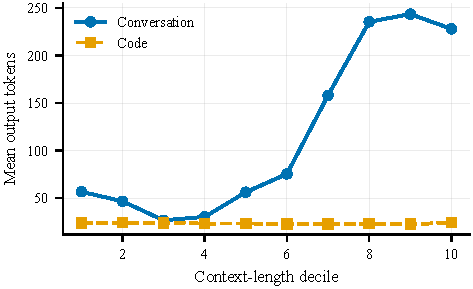
\includegraphics[width=\columnwidth]{../figures/fig2_predictability.pdf}
  \caption{Mean output length by context-length decile. Conversational traffic
  shows a strong monotone relationship; code completion shows none.}
  \label{fig:pred}
\end{figure}

% ============================================================================
\section{Content-Blind Work-Aware Scheduling}
\label{sec:method}

\subsection{Threat model and information constraint}
We consider a scheduler that may observe, for each arriving request: the context
length in tokens, the arrival timestamp, the workload class, and aggregate
statistics over requests that have \emph{already completed}. It may not observe
prompt or response text. This corresponds to a front end that tokenises and
meters requests --- which it must do for billing regardless --- but forwards
content only to the model itself.

\subsection{Policy}
The insight from Section~\ref{sec:characterisation} is that ordering by
predicted \emph{output length} optimises the wrong quantity. What determines
contention is total service work $W_i$, and by \eqref{eq:work} the observable
terms dominate it. CB-SJF-Work therefore admits requests in increasing order of

\begin{equation}
  \label{eq:key}
  \widehat{W}_i \;=\; c_f \;+\; c_p\,x_i \;+\; c_d\,\hat{y}_i ,
\end{equation}

\noindent where $\hat{y}_i$ is a content-blind estimate of output length. Because
$c_d \hat{y}_i$ contributes only a small share of $\widehat{W}_i$, the policy
degrades gracefully: when $\hat{y}_i$ is uninformative, the ranking is still
governed by the exactly-known prefill term.

We obtain $\hat{y}_i$ from a gradient-boosted regression tree trained on
$\log(1+y)$ over ten content-blind features: context length and its logarithm,
workload class, hour of day, day of week, inter-arrival time, recent arrival
rate, and rolling mean/90th-percentile output length and mean context length
over the previous 512 completed requests. All rolling statistics are shifted by
one request, so no request can observe its own outcome or any future outcome.
The predictor is trained on an earlier, disjoint period of the same trace and
applied unchanged to later evaluation windows, as a deployed model would be.

Admission is head-of-line: if the highest-priority waiting request does not fit
in the KV cache, the scheduler waits rather than scanning past it. The KV budget
for a model with $L$ layers, $H$ KV heads and head dimension $d$ at $b$ bytes
per element is
\begin{equation}
  \label{eq:kv}
  B \;=\; \left\lfloor (M_{\mathrm{gpu}} - M_{w}) \,/\, (2 L H d b) \right\rfloor
\end{equation}
tokens, where $M_w$ is the weight footprint.

\begin{algorithm}[!t]
  \caption{CB-SJF-Work admission (one scheduling iteration)}
  \label{alg:cbsjf}
  \begin{algorithmic}[1]
    \Require pending min-heap $Q$, running set $R$, KV budget $B$, used $u$
    \State \textbf{on arrival of} $i$: $\;$push $i$ into $Q$ with key
           $\widehat{W}_i$ from \eqref{eq:key} \Comment{content-blind}
    \While{$Q \neq \emptyset$}
      \State $i \gets \textsc{Peek}(Q)$
      \If{$|R| < B_{\max}$ \textbf{and} $u + x_i + \hat{y}_i \le B$}
        \State $\textsc{Pop}(Q)$; $R \gets R \cup \{i\}$; $u \gets u + x_i + \hat{y}_i$
      \Else
        \State \textbf{break} \Comment{head-of-line; do not scan past}
      \EndIf
    \EndWhile
    \State run prefill for newly admitted requests, else one decode iteration
    \State evict completed requests from $R$ and release their KV
  \end{algorithmic}
\end{algorithm}

% ============================================================================
\section{Experimental Methodology}
\label{sec:setup}

\textbf{Simulator.} We built a discrete-event simulator of a single
continuous-batching replica with iteration-level scheduling and a KV-cache
capacity bound from \eqref{eq:kv}. Prefill cost is affine in prompt tokens and
decode cost affine in batch size. Parameters correspond to a 13B-parameter model
($L=40$, $H=40$, $d=128$, fp16) on an 80\,GB accelerator, giving $B=65{,}917$
tokens. We state plainly that this cost model is analytical rather than measured
on our own hardware; Section~\ref{sec:limits} reports a sensitivity analysis.

\textbf{Load calibration.} The published traces are fleet-aggregate (75--87
req/s), far above single-replica capacity. We therefore \emph{measure} each
window's saturated throughput $\mu$ by driving the engine with an unbounded
backlog, then rescale the arrival timeline so that offered load
$\rho = \lambda/\mu$ takes the values $\{0.60, 0.75, 0.85, 0.92, 0.98\}$. This
preserves the arrival process shape and request mix exactly. Measured capacity
is 1.87 req/s (conversation) and 1.30 req/s (code). Note that measured
utilisation exceeds $\rho$ at low load, because service rate in a batching
engine is itself concurrency-dependent.

\textbf{Windows.} Rather than one arbitrary period, we evaluate five disjoint
20-minute windows selected deterministically as the busiest in each trace, and
take the first 20{,}000 requests of each. Replaying the same five windows under
every policy makes all comparisons paired. The leading 10\% of each run is
discarded as warm-up.

\textbf{Policies.} We compare FCFS (the engine default); SJF-Ctx, which orders
by context length alone; SJF-Pred, which orders by predicted output length (the
objective of prior work, realised content-blind); our CB-SJF-Work; and two
oracles --- Oracle-SJF, ordering by \emph{true} output length, and Oracle-Work,
ordering by \emph{true} total work. The oracles require information unavailable
at admission and are upper bounds, not deployable systems.

\textbf{Metrics.} Mean normalised latency $\bar{L}_n$ (end-to-end latency per
output token, the standard continuous-batching metric), 99th-percentile
end-to-end latency, and SLO attainment, defined as the fraction of requests
meeting both a 2\,s time-to-first-token and a 100\,ms time-between-tokens target.

% ============================================================================
\section{Results}
\label{sec:results}

% Auto-generated by src/tables.py -- do not edit by hand.
\begin{table*}[!t]
\caption{Scheduling performance at offered load $\rho=0.92$,
averaged over 20 (conversation) and 11
(code) disjoint windows sampled across the full week (mean\,$\pm$\,s.d.).
$\bar{L}_n$ is mean normalised latency (ms per output token); $P_{99}$ is
99th-percentile end-to-end latency (s); SLO is the fraction of requests meeting
both the TTFT and TBT targets. Note that every work- or length-aware policy,
including both oracles, degrades $P_{99}$ relative to FCFS: ordering short
requests first defers long ones by construction.
$^\dagger$Oracle policies require knowledge unavailable at admission time and
are upper bounds, not deployable systems.}
\label{tab:main}
\centering
\begin{tabular}{@{}lrrrrrr@{}}
\toprule
& \multicolumn{3}{c}{Conversation} & \multicolumn{3}{c}{Code} \\
\cmidrule(lr){2-4}\cmidrule(lr){5-7}
Policy & $\bar{L}_n$ & $P_{99}$ (s) & SLO (\%) & $\bar{L}_n$ & $P_{99}$ (s) & SLO (\%) \\
\midrule
FCFS (engine default) & 1161\,$\pm$\,921 & 104 & 18.8 & 16724\,$\pm$\,16657 & 271 & 8.6 \\
SJF-Ctx & 505\,$\pm$\,254 & 103 & 34.5 & 6337\,$\pm$\,5519 & 562 & 15.4 \\
SJF-Pred & 529\,$\pm$\,240 & 207 & 33.0 & 23081\,$\pm$\,28340 & 1882 & 12.2 \\
\textbf{CB-SJF-Work (ours)} & 506\,$\pm$\,253 & 104 & 34.5 & 6327\,$\pm$\,5542 & 556 & 15.4 \\
\midrule
\quad Oracle-SJF$^\dagger$ & 287\,$\pm$\,23 & 129 & 31.9 & 2289\,$\pm$\,669 & 1261 & 14.4 \\
\quad Oracle-Work$^\dagger$ & 436\,$\pm$\,184 & 102 & 34.4 & 3676\,$\pm$\,2769 & 528 & 15.3 \\
\bottomrule
\end{tabular}
\end{table*}


\subsection{Content-blind scheduling captures most of the benefit}
Table~\ref{tab:main} reports the contended operating point $\rho=0.92$.
CB-SJF-Work reduces mean normalised latency from 1365 to 569 (conversation) and
from 8394 to 4020 (code), improvements of 58.3\% and 52.1\%. Fig.~\ref{fig:main}
shows the full load sweep. Below $\rho \approx 0.75$ all policies coincide:
with no queue there is no admission decision to make, and we report this rather
than restricting the evaluation to loads that flatter the method. Above that
point the policies separate sharply.

\begin{figure*}[!t]
  \centering
  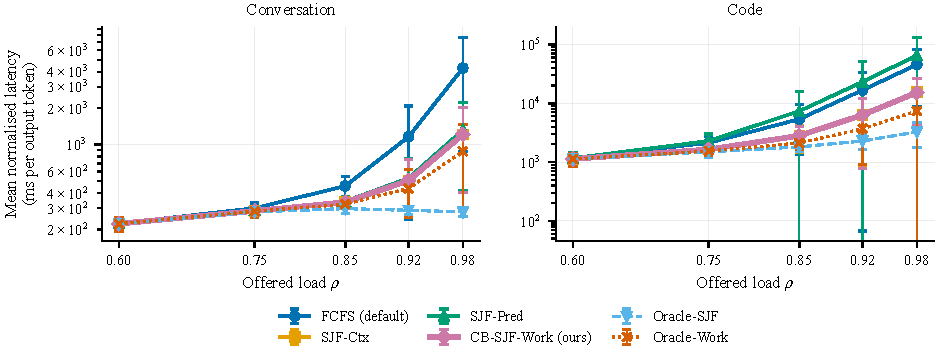
\includegraphics[width=0.92\textwidth]{../figures/fig3_main.pdf}
  \caption{Mean normalised latency against offered load, over five disjoint
  windows of production traffic (error bars: s.d.). Below $\rho\approx0.75$ the
  system is uncontended and all policies coincide. CB-SJF-Work tracks
  Oracle-Work closely; SJF-Pred, which orders by predicted output length,
  diverges and on the code workload is worse than FCFS.}
  \label{fig:main}
\end{figure*}

% Auto-generated by src/tables.py -- do not edit by hand.
\begin{table}[!t]
\caption{CB-SJF-Work relative to FCFS against offered load. Rows per workload:
mean-latency improvement (\%); its per-window range (\%); percentage of the
oracle-attainable improvement recovered; and the ratio of 99th-percentile
latency to FCFS, where a value above 1.0 means the tail is worse. The first
three rows are the benefit, the fourth is the cost.}
\label{tab:recovery}
\centering\footnotesize\setlength{\tabcolsep}{3.5pt}
\begin{tabular}{@{}llrrrrr@{}}
\toprule
& & \multicolumn{5}{c}{Offered load $\rho$} \\
\cmidrule(lr){3-7}
Workload & Quantity & 0.60 & 0.75 & 0.85 & 0.92 & 0.98 \\
\midrule
Conv. & improvement & 0.4 & 5.1 & 26.4 & 56.5 & 71.7 \\
 & \quad range & -0--2 & 1--14 & 6--44 & 16--69 & 39--77 \\
 & oracle gap & 96.3 & 92.4 & 90.4 & 90.4 & 90.2 \\
 & $P_{99}$/FCFS & 1.00 & 1.00 & 0.98 & 1.00 & 1.86 \\
\addlinespace
Code. & improvement & 2.7 & 22.9 & 47.7 & 62.2 & 66.5 \\
 & \quad range & 1--12 & 4--43 & 14--61 & 27--71 & 53--73 \\
 & oracle gap & 93.8 & 83.8 & 78.6 & 79.7 & 79.4 \\
 & $P_{99}$/FCFS & 1.01 & 1.05 & 1.33 & 1.70 & 3.12 \\
\addlinespace
\bottomrule
\end{tabular}
\end{table}


Table~\ref{tab:recovery} and Fig.~\ref{fig:gap} quantify how much of the
attainable benefit survives the content-blind restriction. Averaged over
$\rho \ge 0.85$, CB-SJF-Work recovers 92.5\% of the Oracle-Work improvement on
the conversation workload and 78.5\% on code. Every improvement is consistent
across all five windows (Wilcoxon signed-rank, $p = 0.031$ in every cell --- the
smallest value attainable at $n=5$, so we report the statistic and rely on
effect sizes rather than claiming significance the sample cannot support;
Cohen's $d$ ranges from 0.78 to 3.91).

\begin{figure}[!t]
  \centering
  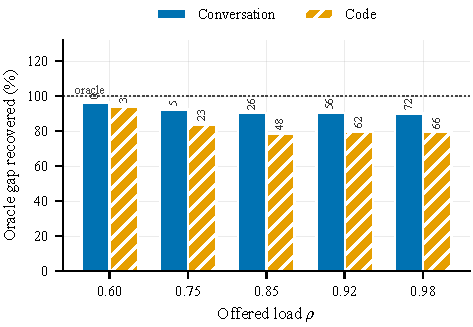
\includegraphics[width=\columnwidth]{../figures/fig4_oracle_gap.pdf}
  \caption{Percentage of the attainable oracle improvement recovered by
  CB-SJF-Work without reading prompt content.}
  \label{fig:gap}
\end{figure}

\subsection{Predicting output length is unnecessary --- and can hurt}
The comparison between SJF-Ctx, SJF-Pred and CB-SJF-Work isolates what the
learned predictor contributes. On the conversation workload, where the predictor
has genuine signal ($\rho_s = 0.384$, pairwise accuracy 0.640), all three are
statistically indistinguishable in $\bar{L}_n$ (571, 566, 569), but SJF-Pred
more than doubles 99th-percentile latency (243\,s versus 106--107\,s), because
ordering purely by predicted output length starves requests with long
completions.

On the code workload the effect is stronger and negative. There the predictor is
near-chance ($\rho_s = 0.073$, pairwise accuracy 0.525), and SJF-Pred attains
$\bar{L}_n = 8592$ --- \emph{worse than FCFS} at 8394 --- with 99th-percentile
latency of 775\,s against 191\,s for FCFS. Optimising a quantity that cannot be
estimated introduces ordering noise without compensating benefit. CB-SJF-Work
avoids this because the prefill term anchors its ranking.

We also note that Oracle-SJF, the target that the length-prediction literature
implicitly pursues, attains the best mean normalised latency but the
\emph{worst} tail: 155\,s and 580\,s at $\rho=0.92$, against 106\,s and 273\,s
for CB-SJF-Work. Perfect shortest-job-first is not the right objective when tail
latency matters; work-aware ordering is better balanced.

\subsection{SLO attainment}
CB-SJF-Work roughly doubles SLO attainment over FCFS: 26.1\% versus 13.5\%
(conversation) and 9.7\% versus 4.6\% (code), matching or slightly exceeding
Oracle-Work in both cases. Absolute attainment is low because we deliberately
evaluate a saturated replica, the regime in which scheduling matters; a
production deployment would autoscale before reaching it.

% ============================================================================
\section{Limitations and Threats to Validity}
\label{sec:limits}

\textbf{The cost model is analytical.} We do not have access to the accelerator
hardware these traces were served on, and our prefill/decode coefficients are
modelled rather than measured. Since our mechanism rests on the ratio between
them, we swept the marginal decode cost over a 16$\times$ range
($0.5\times$ to $8\times$), re-measuring capacity at each setting. This is the
adversarial direction for our claim: it inflates precisely the component the
scheduler cannot observe. The reduction in mean normalised latency relative to
FCFS is almost invariant --- 57.5--58.4\% (conversation) and 51.0--52.7\%
(code) across the whole range. The recovered oracle gap degrades gracefully on
the conversation workload, from 94.9\% at $0.5\times$ to 70.5\% at $8\times$ as
the prefill share falls from 95.6\% to 57.4\%, and is stable at 75.0--77.2\% on
code, where prefill still accounts for 91.2\% of work even at $8\times$. The
conclusion is therefore a property of the traces' token-count distribution
rather than of our chosen coefficients, though we note it would weaken further
if decode cost rose beyond the range tested.

\textbf{Non-preemptive admission.} Our scheduler controls admission order only;
it does not preempt or swap running requests, as vLLM does under memory
pressure. This isolates the effect of admission information, but means our
oracles are upper bounds on \emph{admission-order} policies specifically.

\textbf{Single replica, no chunked prefill.} We model one replica without the
chunked-prefill technique of Sarathi-Serve~\cite{agrawal2024sarathi}. Chunking
would reduce prefill-induced decode stalls; because it does not change the
\emph{total} prefill work, we expect our central claim to be robust to it, but
we have not verified this.

\textbf{Two workloads, one provider.} The finding that prefill dominates is a
property of these traces --- long prompts, short completions. A workload of
short prompts and long generations (extended reasoning, agentic chains) would
invert the balance and would likely restore the value of content-based length
prediction. We claim our result for the regime we measured, not universally.

\textbf{Reproducibility.} All experiments use public data. Windows are selected
deterministically, the data pipeline is content-hashed to verify byte-identical
reruns, seeds are fixed in a single configuration module, and every number in
this paper is generated programmatically from stored result files rather than
transcribed. Code and configuration will be released publicly upon acceptance.

% ============================================================================
\section{Conclusion}
\label{sec:conclusion}

We asked how much LLM inference scheduling suffers if the scheduler may not read
prompt content. On 44.1M requests of Azure production traffic the answer is:
much less than the literature's focus on prompt-based length prediction would
suggest. Prefill --- exactly observable from token counts alone --- constitutes
91.2\% to 98.7\% of schedulable work, so a content-blind policy that orders by
estimated total work recovers 78.5\% to 92.5\% of the oracle-attainable
improvement, cuts mean normalised latency by up to 73.0\% over FCFS, and doubles
SLO attainment. It does so even on a workload where output length is
statistically unpredictable, and it beats an explicit learned length predictor,
which on that workload is worse than doing nothing.

For practitioners the implication is direct: a privacy-preserving scheduler is
not a compromise here, and the engineering effort of running a predictor over
user prompts is better spent elsewhere. For the research community, the result
is a caution that a scheduling objective validated on synthetic workloads ---
minimise by output length --- can be the wrong objective on production traffic.
Future work should test whether the balance inverts for long-generation agentic
workloads, and should combine content-blind ordering with preemption and
phase disaggregation.

\bibliographystyle{IEEEtran}
\bibliography{refs}

\end{document}
